%
% auth: Mattijs Korpershoek
% mail: <mattijs.korpershoek@gmail.com>
%

% {{{1 intro
\section{Technical contributions}
\subsection{Directions}
\begin{FrameWithSubSection}
    \begin{itemize}
        \item Customer features
        \item Open-sourcing a core component
    \end{itemize}
\end{FrameWithSubSection}


% {{{1 Customer features
\subsection{Features for customers}
\begin{FrameWithSubSection}
    \begin{itemize}
        \item More than \emph{80} patches delivered
        \item Code integrated into Intel's code base
        \item Software quality compliant
    \end{itemize}
\end{FrameWithSubSection}

% {{{2 xml validation
\subsubsection{Xml Validation at build time}
\begin{frame}
    \frametitle{XML Validation at build time}
    \begin{itemize}
        \item More than 40 000 lines of XML
        \item More than 500 errors within those files
        \item Validation with XSD files is necessary
    \end{itemize}
\end{frame}

\begin{frame}
    \frametitle{Build generation before}
        \centering
        \includegraphics[height=0.85\textheight]{../../report/src/img/build-generation.pdf}
\end{frame}

\begin{frame}
    \frametitle{Build generation after}
    \centering
    \includegraphics[height=0.85\textheight]{../../report/src/img/build-generation-after.pdf}
\end{frame}

% {{{2 fixed point
\subsubsection{Fixed point parameter improvements}
\begin{frame}
    \frametitle{Fixed point parameter improvements}
    \begin{block}{Fixed point numbers}
        \begin{itemize}
            \item $Qn.m$ notation
                \begin{itemize}
                    \item $n$ : fractional part
                    \item $m$ : integral part
                \end{itemize}
            \item Rounding issues
            \item \lstinline{std::setPrecision()}
            \item Conversion to floating point
        \end{itemize}
    \end{block}
\end{frame}

\begin{frame}
    \frametitle{The problem}
    \begin{minipage}{\textwidth}
        \flushright
        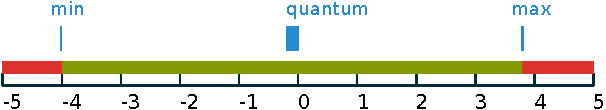
\includegraphics[width=\textwidth]{../../report/src/img/fixedPoint.pdf}
    \end{minipage}
    \begin{minipage}{\textwidth}
        \begin{block}{Example for $Q2.3$}
            \begin{itemize}
                \item $Quantum$ = $2^{-3} = 0.125$
                \item $UpperBound$ = $2^2 - Quantum = 3.875$
                \item $LowerBound$ = $-2^2 = -4$.
            \end{itemize}
        \end{block}
    \end{minipage}
\end{frame}

\begin{frame}
    \frametitle{The problem}
    \lstinputlisting[language=bash]{./code/fixedPoint.bash}
\end{frame}

\begin{frame}
    \frametitle{Behavior description with a test suite}
    \centering
    \includegraphics[height=0.85\textheight]{../../report/src/img/fixedPointProcess.pdf}
\end{frame}

\begin{frame}
    \frametitle{Solution}
    \begin{itemize}
        \item Change \lstinline{std::setPrecision()} argument
        \item Use the fractional part, $m$
        \item More digits to avoid round issues
    \end{itemize}
\end{frame}


% TODO here add results and conclusion
% And code of it working
\begin{frame}
    \frametitle{Results}
    \lstinputlisting[language=bash]{./code/fixedPointOK.bash}
\end{frame}

% {{{1 Opensourcing
\subsection{Open-sourcing the Parameter-framework}
\subsubsection{Context}
\begin{FrameWithSubSection}
    \begin{block}{Why open-sourcing this component?}
        \begin{itemize}
            \item Core component of Intel audio HAL
            \item Middleware standard
            \item Visibility
        \end{itemize}
    \end{block}
\end{FrameWithSubSection}

\subsubsection{Documentation}
\begin{frame}
    \frametitle{Newcomer documentation}
    \centering
    \begin{block}{Is the component ready for open-sourcing?}
        \begin{itemize}
            \item Code review and study
            \item Documentation for external contributors
            \item More than 450 lines of documentation
        \end{itemize}
    \end{block}
\end{frame}

\begin{frame}
    \frametitle{Newcomer documentation illustration}
    \centering
    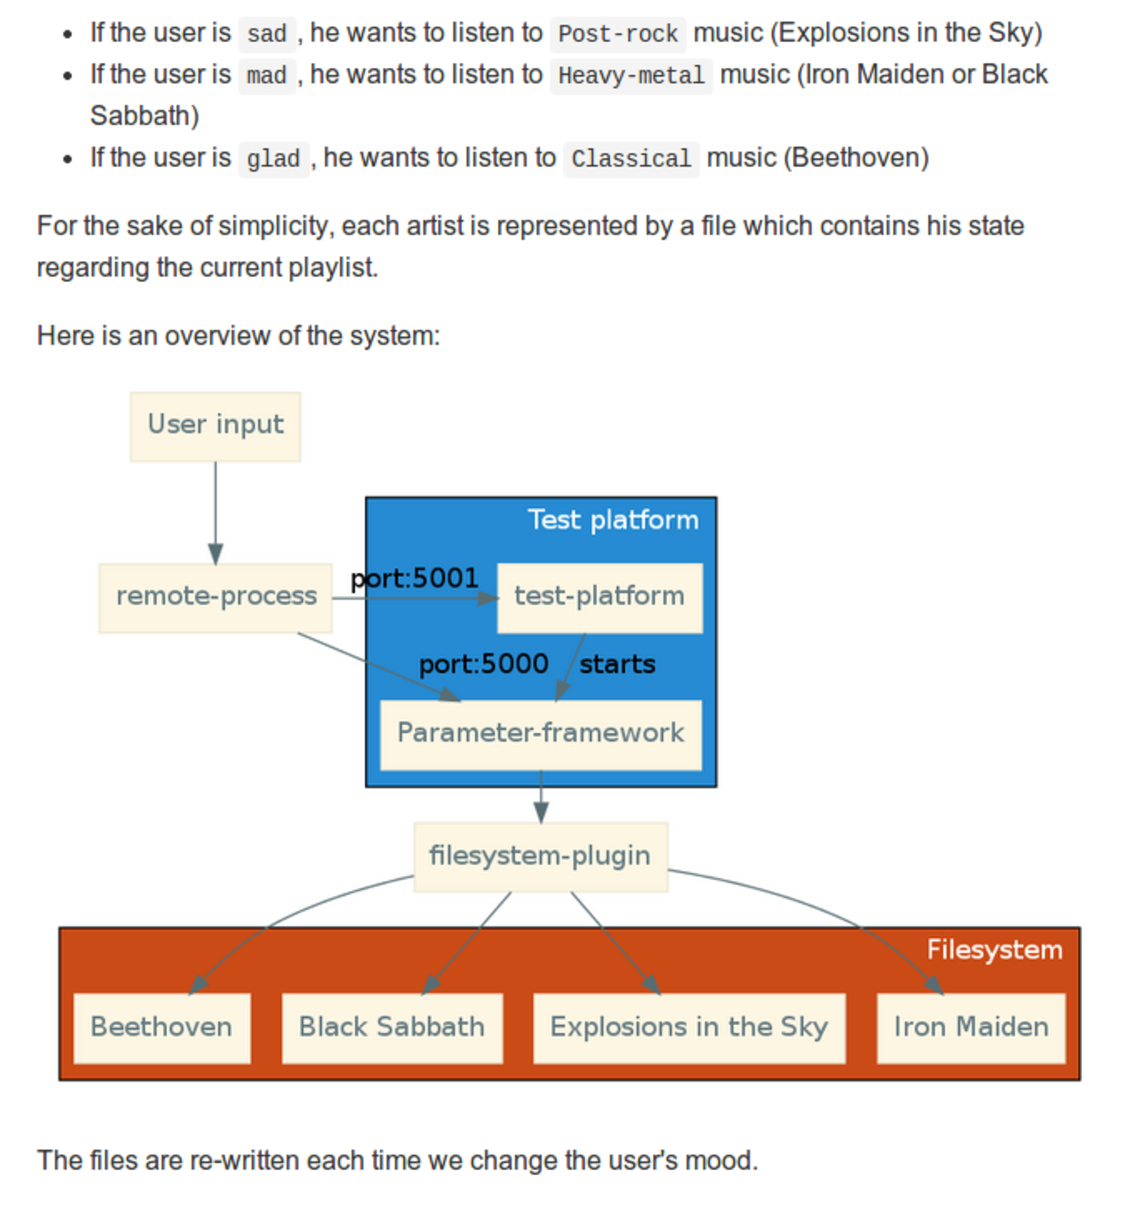
\includegraphics[height=0.85\textheight]{../../report/src/img/tutos.pdf}
\end{frame}

\subsubsection{Branch sync process}
\begin{frame}
    \frametitle{Branch sync process}
    \begin{block}{How to open-source the component?}
        \begin{itemize}
            \item Ensure external contributions are of quality
            \item Avoid maintenance of 2 divergent code bases
            \item Ensure no confidential information is exposed
        \end{itemize}
    \end{block}
\end{frame}

\begin{frame}
    \frametitle{Branch sync process}
    \centering
    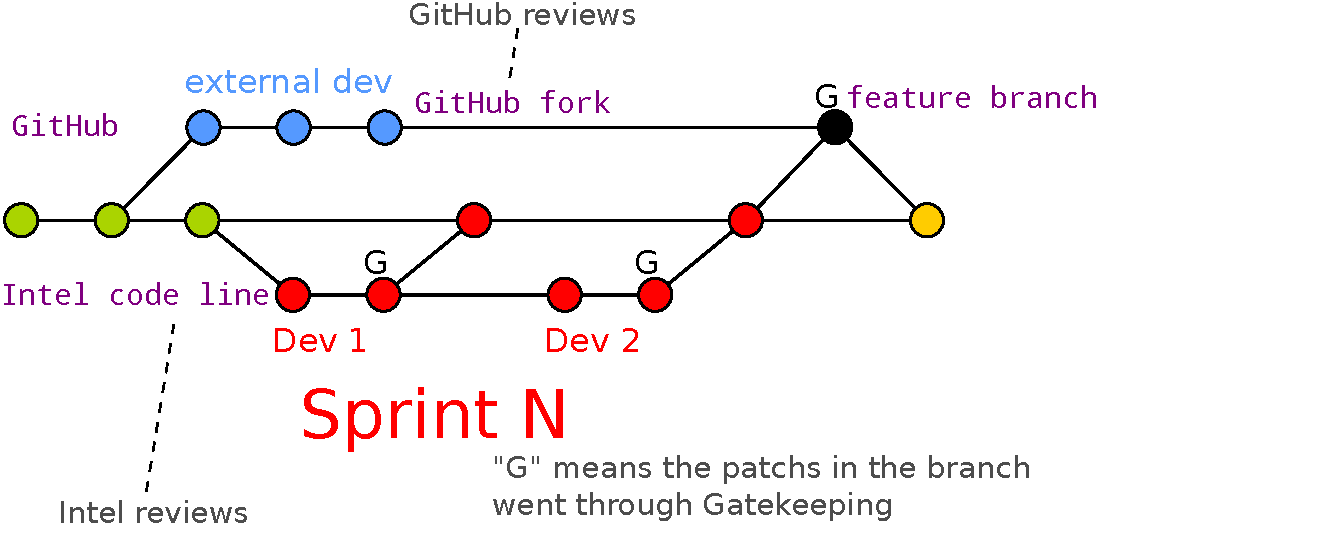
\includegraphics[width=\textwidth]{../../report/src/img/branches-process.pdf}
\end{frame}

\subsubsection{Open-sources projects}
\begin{frame}
    \frametitle{Projects which are open-source}
    \begin{itemize}
        \item Parameter-framework core
        \item Parameter-framework ALSA plugin
        \item Parameter-framework filesystem plugin
    \end{itemize}
\end{frame}

\begin{frame}
    \frametitle{GitHub top contributors}
    \centering
    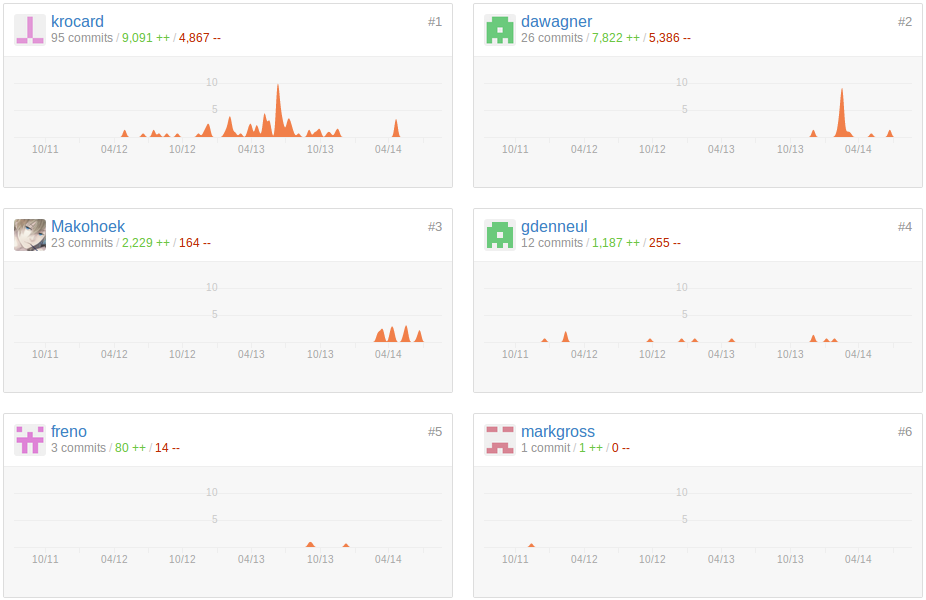
\includegraphics[width=\textwidth]{../../report/src/img/statsGitHub.png}
\end{frame}

